%%
% ------------------------------------------------------------------------------
% OraDBA - Oracle Database Infrastructure and Security, 5630 Muri, Switzerland
% ------------------------------------------------------------------------------
% Name.......: oradba.tex
% Author.....: Stefan Oehrli (oes) stefan.oehrli@oradba.ch
% Editor.....: Stefan Oehrli
% Date.......: 2025.09.02
% Revision...: --
% Purpose....: LaTeX template for pandoc
% Notes......: This is a LaTeX template for converting documents with Pandoc. 
%              Mainly for converting Markdown files into PDF documents. Adjustments
%              in the conversion and customisation of the PDF e.g., geometry,
%              colors, font, ToC, title etc. are made with the help of a YAML
%              meta block or a metadata file.
%
%              Detailed information can be found under the following links:
%              - https://pandoc.org/
%              - https://github.com/oehrlis/pandoc_template
%              - https://github.com/oehrlis/docker-pandoc
%
% Reference..: https://github.com/Wandmalfarbe/pandoc-latex-template
% License....: Apache License Version 2.0, January 2004 as shown
%              at http://www.apache.org/licenses/
% ------------------------------------------------------------------------------
%%

% Options for packages loaded elsewhere
\PassOptionsToPackage{unicode}{hyperref}
\PassOptionsToPackage{hyphens}{url}
\PassOptionsToPackage{dvipsnames,svgnames,x11names,table}{xcolor}
%
\documentclass[
  a4paper,
  ,captions=tableheading
]{scrartcl}
\usepackage{amsmath,amssymb}
% Use setspace anyway because we change the default line spacing.
% The spacing is changed early to affect the titlepage and the TOC.
\usepackage{setspace}
\setstretch{1.2}
\usepackage{iftex}
\ifPDFTeX
  \usepackage[T1]{fontenc}
  \usepackage[utf8]{inputenc}
  \usepackage{textcomp} % provide euro and other symbols
\else % if luatex or xetex
  \usepackage{unicode-math} % this also loads fontspec
  \defaultfontfeatures{Scale=MatchLowercase}
  \defaultfontfeatures[\rmfamily]{Ligatures=TeX,Scale=1}
\fi
\usepackage{lmodern}
\ifPDFTeX\else
  % xetex/luatex font selection
  \setmainfont[]{Arial}
  \setsansfont[]{Arial}
  \setmonofont[]{Courier New}
\fi
% Use upquote if available, for straight quotes in verbatim environments
\IfFileExists{upquote.sty}{\usepackage{upquote}}{}
\IfFileExists{microtype.sty}{% use microtype if available
  \usepackage[]{microtype}
  \UseMicrotypeSet[protrusion]{basicmath} % disable protrusion for tt fonts
}{}
\makeatletter
\@ifundefined{KOMAClassName}{% if non-KOMA class
  \IfFileExists{parskip.sty}{%
    \usepackage{parskip}
  }{% else
    \setlength{\parindent}{0pt}
    \setlength{\parskip}{6pt plus 2pt minus 1pt}}
}{% if KOMA class
  \KOMAoptions{parskip=half}}
\makeatother
\usepackage{xcolor}
\definecolor{default-linkcolor}{HTML}{A50000}
\definecolor{default-filecolor}{HTML}{A50000}
\definecolor{default-citecolor}{HTML}{4077C0}
\definecolor{default-urlcolor}{HTML}{4077C0}
\definecolor{title-color}{HTML}{000000}
\definecolor{subtitle-color}{HTML}{A100FF}
\usepackage[top=2.54cm,bottom=2.54cm,left=2.54cm,right=2.54cm]{geometry}
\usepackage[export]{adjustbox}
\usepackage{graphicx}
\usepackage{listings}
\newcommand{\passthrough}[1]{#1}
\lstset{defaultdialect=[5.3]Lua}
\lstset{defaultdialect=[x86masm]Assembler}
\usepackage{etoolbox}
\BeforeBeginEnvironment{lstlisting}{\par\noindent\begin{minipage}{\linewidth}}
\AfterEndEnvironment{lstlisting}{\end{minipage}\par\addvspace{\topskip}}
\usepackage{longtable,tabularx,booktabs,array,ragged2e}
\setlength{\extrarowheight}{1pt}
\usepackage{calc} % for calculating minipage widths
% Correct order of tables after \paragraph or \subparagraph
\usepackage{etoolbox}
\makeatletter
\patchcmd\longtable{\par}{\if@noskipsec\mbox{}\fi\par}{}{}
\makeatother
% Allow footnotes in longtable head/foot
\IfFileExists{footnotehyper.sty}{\usepackage{footnotehyper}}{\usepackage{footnote}}
\makesavenoteenv{longtable}
% add backlinks to footnote references, cf. https://tex.stackexchange.com/questions/302266/make-footnote-clickable-both-ways
\usepackage{footnotebackref}
\usepackage{graphicx}
\makeatletter
\def\maxwidth{\ifdim\Gin@nat@width>\linewidth\linewidth\else\Gin@nat@width\fi}
\def\maxheight{\ifdim\Gin@nat@height>\textheight\textheight\else\Gin@nat@height\fi}
\makeatother
% Scale images if necessary, so that they will not overflow the page
% margins by default, and it is still possible to overwrite the defaults
% using explicit options in \includegraphics[width, height, ...]{}
\setkeys{Gin}{width=\maxwidth,height=\maxheight,keepaspectratio}
% Set default figure placement to htbp
\makeatletter
% Make use of float-package and set default placement for figures to H.
% The option H means 'PUT IT HERE' (as  opposed to the standard h option which means 'You may put it here if you like').
\usepackage{float}
\floatplacement{figure}{H}
\makeatother
\setlength{\emergencystretch}{3em} % prevent overfull lines
\providecommand{\tightlist}{%
  \setlength{\itemsep}{0pt}\setlength{\parskip}{0pt}}
\setcounter{secnumdepth}{5}
% former header from metadata
\setcounter{page}{0}
\usepackage{awesomebox}
\usepackage{sectsty}
\sectionfont{\clearpage}

\ifLuaTeX
\usepackage[bidi=basic]{babel}
\else
\usepackage[bidi=default]{babel}
\fi
\babelprovide[main,import]{english}
\ifPDFTeX
\else
\babelfont{rm}[]{Arial}
\fi
% get rid of language-specific shorthands (see #6817):
\let\LanguageShortHands\languageshorthands
\def\languageshorthands#1{}
\definecolor{purple}{HTML}{A100FF}
\ifLuaTeX
  \usepackage{selnolig}  % disable illegal ligatures
\fi
\IfFileExists{bookmark.sty}{\usepackage{bookmark}}{\usepackage{hyperref}}
\IfFileExists{xurl.sty}{\usepackage{xurl}}{} % add URL line breaks if available
% -- Pandoc >= 2.19 image wrapper macro ---------------------------------------
% Ensures images are constrained to page width/height when Pandoc wraps them in
% \pandocbounded{...}. Safe even if graphicx/adjustbox were already loaded.
\makeatletter
\@ifpackageloaded{graphicx}{}{\usepackage{graphicx}}
\@ifpackageloaded{adjustbox}{}{\usepackage{adjustbox}}
\makeatother
\providecommand{\pandocbounded}[1]{%
  \begin{adjustbox}{max size={\linewidth}{\textheight}}#1\end{adjustbox}%
}
% -----------------------------------------------------------------------------

\urlstyle{same}

% Enable strike-through (\st) without redefining \emph or \underline
\IfFileExists{soulutf8.sty}{\usepackage{soulutf8}}{\usepackage{soul}}

% Make \sout work even without ulem
\providecommand{\sout}[1]{\st{#1}}

\hypersetup{
  pdftitle={OraDBA Markdown Doc Template},
  pdfauthor={Stefan Oehrli},
  pdflang={en},
  colorlinks=true,
  linkcolor={purple},
  filecolor={purple},
  citecolor={default-citecolor},
  urlcolor={purple},
  breaklinks=true,
  pdfcreator={LaTeX via pandoc with the OraDBA template}}
\title{OraDBA Markdown Doc Template}
\usepackage{etoolbox}
\makeatletter
\providecommand{\subtitle}[1]{% add subtitle to \maketitle
  \apptocmd{\@title}{\par {\large #1 \par}}{}{}
}
\makeatother
\subtitle{A template for markdown based documentation}
\author{Stefan Oehrli}
\date{}

%%
%% added
%%


%
% for the background color of the title page
%
\usepackage{pagecolor}
\usepackage{afterpage}

%
% break urls
%
\PassOptionsToPackage{hyphens}{url}

%
% When using babel or polyglossia with biblatex, loading csquotes is recommended
% to ensure that quoted texts are typeset according to the rules of your main language.
%
\usepackage{csquotes}

%
% captions
%
\definecolor{caption-color}{HTML}{777777}
\usepackage[font={stretch=1.2}, textfont={color=caption-color}, position=top, skip=4mm, labelfont=bf, singlelinecheck=false, justification=raggedright]{caption}
\setcapindent{0em}

%
% blockquote
%
\definecolor{blockquote-border}{RGB}{221,221,221}
\definecolor{blockquote-text}{RGB}{119,119,119}
\usepackage{mdframed}
\newmdenv[rightline=false,bottomline=false,topline=false,linewidth=3pt,linecolor=blockquote-border,skipabove=\parskip]{customblockquote}
\renewenvironment{quote}{\begin{customblockquote}\list{}{\rightmargin=0em\leftmargin=0em}%
\item\relax\color{blockquote-text}\ignorespaces}{\unskip\unskip\endlist\end{customblockquote}}

%
% Source Sans Pro as the default font family
% Source Code Pro for monospace text
%
% 'default' option sets the default
% font family to Source Sans Pro, not \sfdefault.
%
\ifnum 0\ifxetex 1\fi\ifluatex 1\fi=0 % if pdftex
    \usepackage[default]{sourcesanspro}
  \usepackage{sourcecodepro}
  \else % if not pdftex
    \fi

%
% heading color
%
\definecolor{heading-color}{RGB}{40,40,40}
\addtokomafont{section}{\color{heading-color}}
% When using the classes report, scrreprt, book,
% scrbook or memoir, uncomment the following line.
%\addtokomafont{chapter}{\color{heading-color}}

%
% variables for title, author and date
%
\usepackage{titling}
\title{OraDBA Markdown Doc Template}
\author{Stefan Oehrli}
\date{}

%
% tables
%

\definecolor{table-row-color}{HTML}{F5F5F5}
\definecolor{table-rule-color}{HTML}{999999}

%\arrayrulecolor{black!40}
\arrayrulecolor{table-rule-color}     % color of \toprule, \midrule, \bottomrule
\setlength\heavyrulewidth{0.3ex}      % thickness of \toprule, \bottomrule
\renewcommand{\arraystretch}{1.3}     % spacing (padding)


%
% remove paragraph indention
%
\setlength{\parindent}{0pt}
\setlength{\parskip}{6pt plus 2pt minus 1pt}
\setlength{\emergencystretch}{3em}  % prevent overfull lines

%
%
% Listings
%
%


%
% general listing colors
%
\definecolor{listing-background}{HTML}{F7F7F7}
\definecolor{listing-rule}{HTML}{B3B2B3}
\definecolor{listing-numbers}{HTML}{B3B2B3}
\definecolor{listing-text-color}{HTML}{000000}
\definecolor{listing-keyword}{HTML}{435489}
\definecolor{listing-keyword-2}{HTML}{1284CA} % additional keywords
\definecolor{listing-keyword-3}{HTML}{9137CB} % additional keywords
\definecolor{listing-identifier}{HTML}{435489}
\definecolor{listing-string}{HTML}{00999A}
\definecolor{listing-comment}{HTML}{8E8E8E}

\lstdefinestyle{eisvogel_listing_style}{
  language         = java,
  xleftmargin      = 0.6em,
  framexleftmargin = 0.4em,
  backgroundcolor  = \color{listing-background},
  basicstyle       = \color{listing-text-color}\linespread{1.0}%
                      \lst@ifdisplaystyle%
                      \scriptsize%
                      \fi\ttfamily{},
  breaklines       = true,
  frame            = single,
  framesep         = 0.19em,
  rulecolor        = \color{listing-rule},
  frameround       = ffff,
  tabsize          = 4,
  numberstyle      = \color{listing-numbers},
  aboveskip        = 1.0em,
  belowskip        = 0.1em,
  abovecaptionskip = 0em,
  belowcaptionskip = 1.0em,
  keywordstyle     = {\color{listing-keyword}\bfseries},
  keywordstyle     = {[2]\color{listing-keyword-2}\bfseries},
  keywordstyle     = {[3]\color{listing-keyword-3}\bfseries\itshape},
  sensitive        = true,
  identifierstyle  = \color{listing-identifier},
  commentstyle     = \color{listing-comment},
  stringstyle      = \color{listing-string},
  showstringspaces = false,
  escapeinside     = {/*@}{@*/}, % Allow LaTeX inside these special comments
  literate         =
  {á}{{\'a}}1 {é}{{\'e}}1 {í}{{\'i}}1 {ó}{{\'o}}1 {ú}{{\'u}}1
  {Á}{{\'A}}1 {É}{{\'E}}1 {Í}{{\'I}}1 {Ó}{{\'O}}1 {Ú}{{\'U}}1
  {à}{{\`a}}1 {è}{{\`e}}1 {ì}{{\`i}}1 {ò}{{\`o}}1 {ù}{{\`u}}1
  {À}{{\`A}}1 {È}{{\`E}}1 {Ì}{{\`I}}1 {Ò}{{\`O}}1 {Ù}{{\`U}}1
  {ä}{{\"a}}1 {ë}{{\"e}}1 {ï}{{\"i}}1 {ö}{{\"o}}1 {ü}{{\"u}}1
  {Ä}{{\"A}}1 {Ë}{{\"E}}1 {Ï}{{\"I}}1 {Ö}{{\"O}}1 {Ü}{{\"U}}1
  {â}{{\^a}}1 {ê}{{\^e}}1 {î}{{\^i}}1 {ô}{{\^o}}1 {û}{{\^u}}1
  {Â}{{\^A}}1 {Ê}{{\^E}}1 {Î}{{\^I}}1 {Ô}{{\^O}}1 {Û}{{\^U}}1
  {œ}{{\oe}}1 {Œ}{{\OE}}1 {æ}{{\ae}}1 {Æ}{{\AE}}1 {ß}{{\ss}}1
  {ç}{{\c c}}1 {Ç}{{\c C}}1 {ø}{{\o}}1 {å}{{\r a}}1 {Å}{{\r A}}1
  {€}{{\EUR}}1 {£}{{\pounds}}1 {«}{{\guillemotleft}}1
  {»}{{\guillemotright}}1 {ñ}{{\~n}}1 {Ñ}{{\~N}}1 {¿}{{?`}}1
  {…}{{\ldots}}1 {≥}{{>=}}1 {≤}{{<=}}1 {„}{{\glqq}}1 {“}{{\grqq}}1
  {”}{{''}}1
}
\lstset{style=eisvogel_listing_style}

%
% Java (Java SE 12, 2019-06-22)
%
\lstdefinelanguage{Java}{
  morekeywords={
    % normal keywords (without data types)
    abstract,assert,break,case,catch,class,continue,default,
    do,else,enum,exports,extends,final,finally,for,if,implements,
    import,instanceof,interface,module,native,new,package,private,
    protected,public,requires,return,static,strictfp,super,switch,
    synchronized,this,throw,throws,transient,try,volatile,while,
    % var is an identifier
    var
  },
  morekeywords={[2] % data types
    % primitive data types
    boolean,byte,char,double,float,int,long,short,
    % String
    String,
    % primitive wrapper types
    Boolean,Byte,Character,Double,Float,Integer,Long,Short
    % number types
    Number,AtomicInteger,AtomicLong,BigDecimal,BigInteger,DoubleAccumulator,DoubleAdder,LongAccumulator,LongAdder,Short,
    % other
    Object,Void,void
  },
  morekeywords={[3] % literals
    % reserved words for literal values
    null,true,false,
  },
  sensitive,
  morecomment  = [l]//,
  morecomment  = [s]{/*}{*/},
  morecomment  = [s]{/**}{*/},
  morestring   = [b]",
  morestring   = [b]',
}

\lstdefinelanguage{XML}{
  morestring      = [b]",
  moredelim       = [s][\bfseries\color{listing-keyword}]{<}{\ },
  moredelim       = [s][\bfseries\color{listing-keyword}]{</}{>},
  moredelim       = [l][\bfseries\color{listing-keyword}]{/>},
  moredelim       = [l][\bfseries\color{listing-keyword}]{>},
  morecomment     = [s]{<?}{?>},
  morecomment     = [s]{<!--}{-->},
  commentstyle    = \color{listing-comment},
  stringstyle     = \color{listing-string},
  identifierstyle = \color{listing-identifier}
}

%
% header and footer
%
\usepackage{scrlayer-scrpage}
\KOMAoptions{
   headsepline = false,
   footsepline = true,
   plainfootsepline = true,
}
\newpairofpagestyles{eisvogel-header-footer}{
  \clearpairofpagestyles
  \ihead*{}
  \chead*{}
  \ohead*{}
  \ifoot*{Copyright © 2023 Accenture. All rights reserved.}
  \cfoot*{}
  \ofoot*{\thepage}
  \addtokomafont{pageheadfoot}{\upshape}
}
\pagestyle{eisvogel-header-footer}



\makeatletter
\@ifpackageloaded{ulem}{%
  % If someone loaded ulem anyway, restore the original underline commands
  \let\underline\UL@orig@underline
  \let\underbar\UL@orig@underbar
}{}
\makeatother

%%
%% end added
%%

\begin{document}

%%
%% begin titlepage
%%
\begin{titlepage}
\newgeometry{top=2.54cm,bottom=2.54cm,left=2.54cm,right=2.54cm}
\newcommand{\colorRule}[3][black]{\textcolor[HTML]{#1}{\rule{#2}{#3}}}
\begin{flushleft}
\noindent
\\[-1em]
\color[HTML]{000000}
\makebox[0pt][l]{\colorRule[435488]{1.3\textwidth}{0pt}}
\par
\noindent

{
  \setstretch{1.4}
  \vfill
  \noindent {\Huge \textbf{\textbf{\color{title-color}OraDBA Markdown
Doc Template}}}
    \vskip 1em
  {\Large \textbf{\color{subtitle-color}A template for markdown based
documentation}}
    \vskip 0.5em
  \text{\today, Version 0.0.3 }\\
  \noindent {\textsf{Stefan Oehrli}}
  \vfill
}

\noindent

\includegraphics[width=35mm, right]{sample/logo.png}

\textsf{}
\end{flushleft}
\end{titlepage}
\restoregeometry
\pagenumbering{arabic} 

%%
%% end titlepage
%%

% \maketitle


\renewcommand*\contentsname{Table of Contents}
{
\hypersetup{linkcolor=}
\setcounter{tocdepth}{2}
\tableofcontents
\newpage
}
\listoftables
\section{Formatting Examples}\label{formatting-examples}

\subsection{Basic Syntax}\label{basic-syntax}

These are the elements outlined in John Gruber's original design
document. All Markdown applications support these elements.

\subsubsection{Heading}\label{heading}

Headings are created with a \passthrough{\lstinline!\#!}. Where the
number of \passthrough{\lstinline!\#!} corresponds to the level of the
heading.

\begin{lstlisting}
# This is an <h1> tag
## This is an <h2> tag
### This is an <h3> tag
\end{lstlisting}

\subsubsection{Emphasis}\label{emphasis}

\begin{lstlisting}
*This text will be italic*
_This will also be italic_

**This text will be bold**
__This will also be bold__

_You **can** combine them_
\end{lstlisting}

\emph{This text will be italic} \emph{This will also be italic}

\textbf{This text will be bold} \textbf{This will also be bold}

\emph{You \textbf{can} combine them}

\subsubsection{Blockquote}\label{blockquote}

\begin{lstlisting}
> blockquote
\end{lstlisting}

\begin{quote}
blockquote
\end{quote}

\subsubsection{Ordered List}\label{ordered-list}

\begin{enumerate}
\def\labelenumi{\arabic{enumi}.}
\tightlist
\item
  First item
\item
  Second item
\item
  Third item
\end{enumerate}

\subsubsection{Unordered List}\label{unordered-list}

\begin{itemize}
\tightlist
\item
  First item
\item
  Second item
\item
  Third item
\end{itemize}

\subsubsection{Code}\label{code}

\passthrough{\lstinline!code!}

\subsubsection{Horizontal Rule}\label{horizontal-rule}

\begin{center}\rule{0.5\linewidth}{0.5pt}\end{center}

\subsubsection{Link}\label{link}

\href{https://www.example.com}{title}

\subsubsection{Image}\label{image}

\begin{figure}
\centering
\pandocbounded{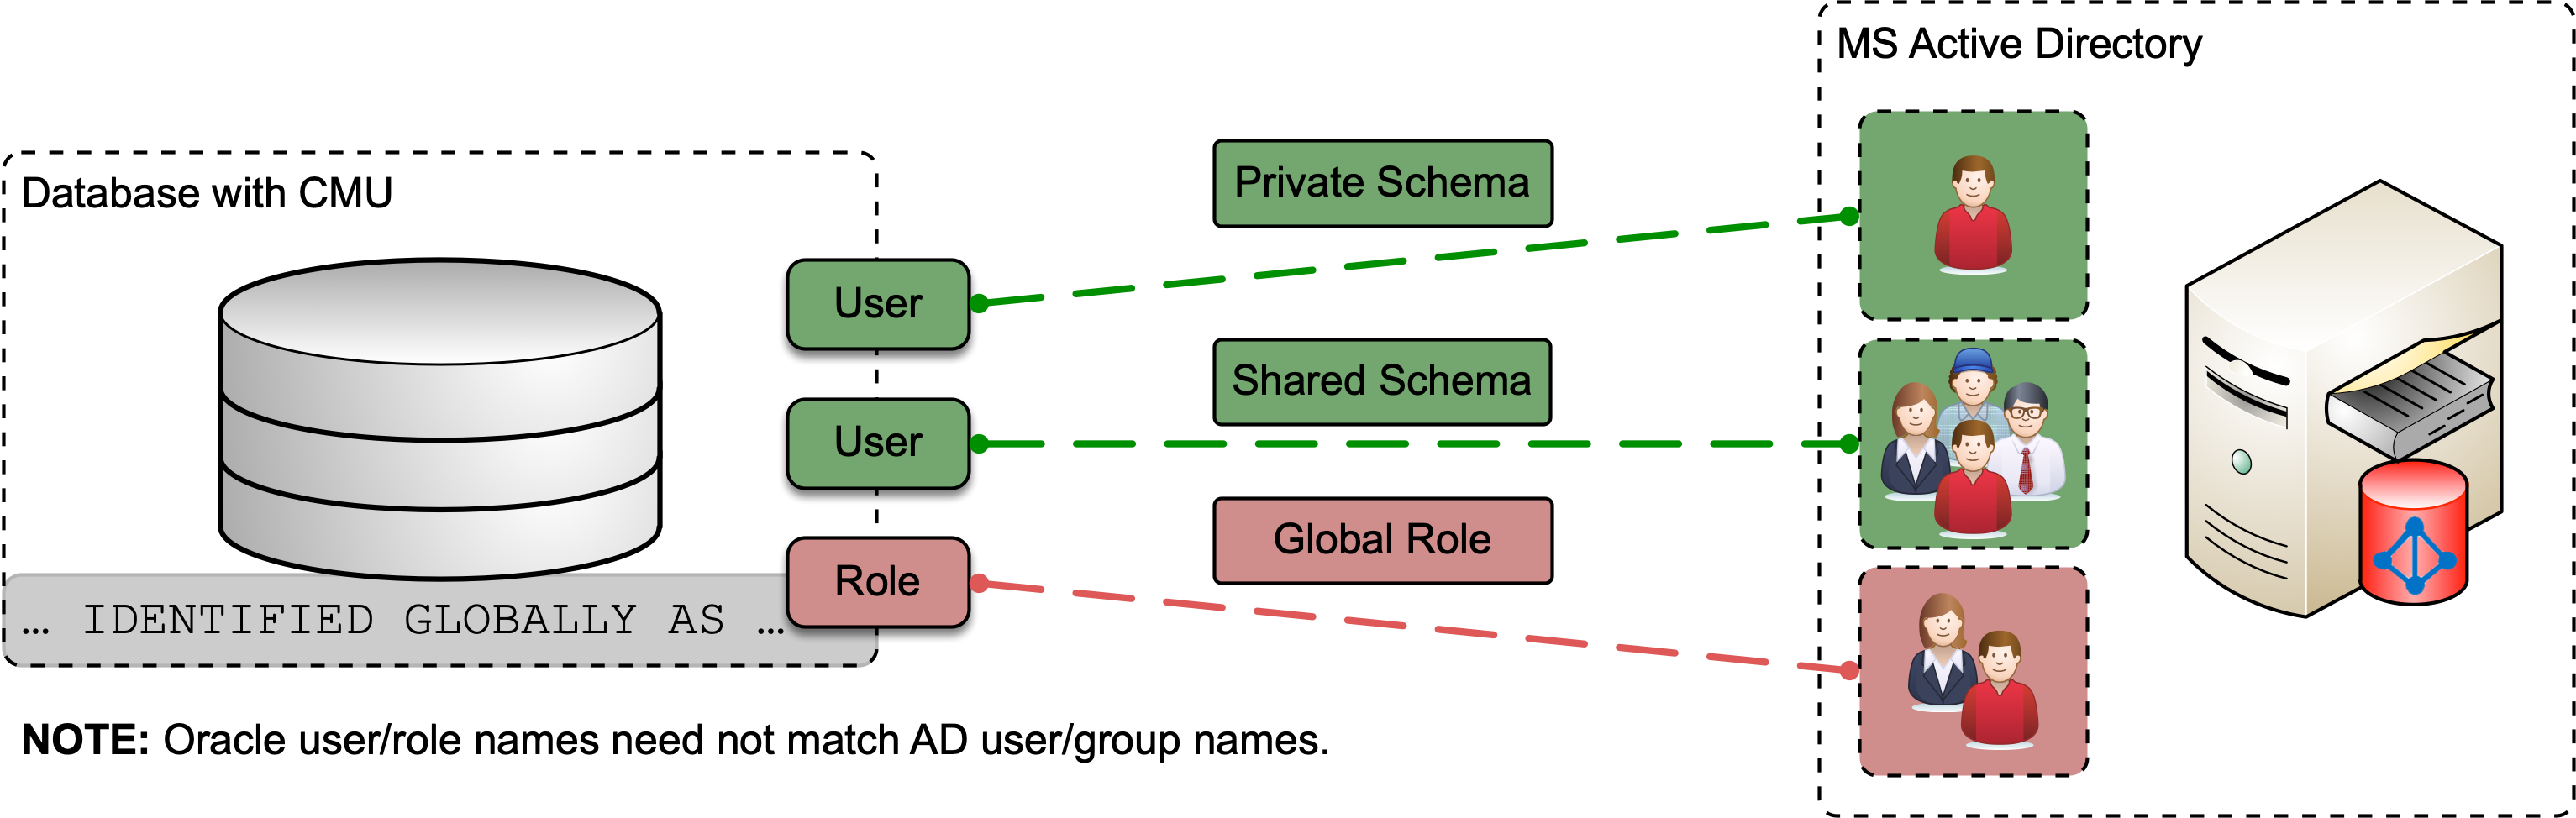
\includegraphics[keepaspectratio,alt={``Oracle Centrally Managed Users Overview''}]{CMU_overview.png}}
\caption{``Oracle Centrally Managed Users Overview''}
\end{figure}

\subsection{Extended Syntax}\label{extended-syntax}

These elements extend the basic syntax by adding additional features.
Not all Markdown applications support these elements.

\subsubsection{Table}\label{table}

\begin{longtable}[]{@{}ll@{}}
\toprule\noalign{}
Syntax & Description \\
\midrule\noalign{}
\endhead
\bottomrule\noalign{}
\endlastfoot
Header & Title \\
Paragraph & Text \\
\end{longtable}

\subsubsection{Fenced Code Block}\label{fenced-code-block}

\begin{lstlisting}
{
  "firstName": "John",
  "lastName": "Smith",
  "age": 25
}
\end{lstlisting}

\subsubsection{Footnote}\label{footnote}

Here's a sentence with a footnote. \footnote{This is the footnote.}

\subsubsection{Heading ID}\label{heading-id}

\subsubsection{My Great Heading}\label{custom-id}

\subsubsection{Definition List}\label{definition-list}

\begin{description}
\tightlist
\item[term]
definition For a list of all available boxes and options visit theFor a
list of all available boxes and options visit theFor a list of all
available boxes and options visit the
\end{description}

\subsubsection{Strikethrough}\label{strikethrough}

\st{The world is flat.}

\subsubsection{Task List}\label{task-list}

\begin{itemize}
\tightlist
\item[$\boxtimes$]
  Write the press release
\item[$\square$]
  Update the website
\item[$\square$]
  Contact the media
\end{itemize}

\subsection{Box Types}\label{box-types}

For a list of all available boxes and options visit the
\href{https://ctan.org/pkg/awesomebox}{\passthrough{\lstinline!awesomebox!}
documentation}.

\begin{lstlisting}
::: note
**Note** Lorem ipsum dolor ...
:::
\end{lstlisting}

\begin{noteblock}
Lorem ipsum dolor sit amet, consectetur adipiscing elit. Nam aliquet
libero quis lectus elementum fermentum.

Fusce aliquet augue sapien, non efficitur mi ornare sed. Morbi at dictum
felis. Pellentesque tortor lacus, semper et neque vitae, egestas commodo
nisl.
\end{noteblock}

\begin{lstlisting}
::: tip
**Tip** Lorem ipsum dolor ...
:::
\end{lstlisting}

\begin{tipblock}
\textbf{Tip} Lorem ipsum dolor sit amet, consectetur adipiscing elit.
Nam aliquet libero quis lectus elementum fermentum.

Fusce aliquet augue sapien, non efficitur mi ornare sed. Morbi at dictum
felis. Pellentesque tortor lacus, semper et neque vitae, egestas commodo
nisl.
\end{tipblock}

\begin{lstlisting}
::: warning
**Warning** Lorem ipsum dolor ...
:::
\end{lstlisting}

\begin{warningblock}
\textbf{Warning} Lorem ipsum dolor sit amet, consectetur adipiscing
elit. Nam aliquet libero quis lectus elementum fermentum.

Fusce aliquet augue sapien, non efficitur mi ornare sed. Morbi at dictum
felis. Pellentesque tortor lacus, semper et neque vitae, egestas commodo
nisl.
\end{warningblock}

\begin{lstlisting}
::: warning
**Caution** Lorem ipsum dolor ...
:::
\end{lstlisting}

\begin{cautionblock}
\textbf{Caution} Lorem ipsum dolor sit amet, consectetur adipiscing
elit. Nam aliquet libero quis lectus elementum fermentum.

Fusce aliquet augue sapien, non efficitur mi ornare sed. Morbi at dictum
felis. Pellentesque tortor lacus, semper et neque vitae, egestas commodo
nisl.
\end{cautionblock}

\begin{lstlisting}
::: important
**Important** Lorem ipsum dolor ...
:::
\end{lstlisting}

\begin{importantblock}
\textbf{Important} Lorem ipsum dolor sit amet, consectetur adipiscing
elit. Nam aliquet libero quis lectus elementum fermentum.

Fusce aliquet augue sapien, non efficitur mi ornare sed. Morbi at dictum
felis. Pellentesque tortor lacus, semper et neque vitae, egestas commodo
nisl.
\end{importantblock}

Markdown formatting inside the environments is supported.

\begin{importantblock}
\textbf{Lorem ipsum dolor} sit amet,
\passthrough{\lstinline!consectetur adipiscing!} elit.

\begin{lstlisting}[language=Java]
if(args.length < 2) {
    System.out.println("Lorem ipsum dolor sit amet");
}
\end{lstlisting}

\emph{Nam aliquet libero quis lectus elementum fermentum.}
\end{importantblock}

\begin{importantblock}
\textbf{OraDBA} Lorem ipsum dolor sit amet, consectetur adipiscing elit.
Nam aliquet libero quis lectus elementum fermentum.

Fusce aliquet augue sapien, non efficitur mi ornare sed. Morbi at dictum
felis. Pellentesque tortor lacus, semper et neque vitae, egestas commodo
nisl.
\end{importantblock}

\begin{importantblock}
\textbf{OraDBA} Lorem ipsum dolor sit amet, consectetur adipiscing elit.
Nam aliquet libero quis lectus elementum fermentum.

Fusce aliquet augue sapien, non efficitur mi ornare sed. Morbi at dictum
felis. Pellentesque tortor lacus, semper et neque vitae, egestas commodo
nisl.
\end{importantblock}

\end{document}